\documentclass[10pt]{article}
\usepackage{tmlr}

%%%%% NEW MATH DEFINITIONS %%%%%

\usepackage{amsmath,amsfonts,bm}

% Mark sections of captions for referring to divisions of figures
\newcommand{\figleft}{{\em (Left)}}
\newcommand{\figcenter}{{\em (Center)}}
\newcommand{\figright}{{\em (Right)}}
\newcommand{\figtop}{{\em (Top)}}
\newcommand{\figbottom}{{\em (Bottom)}}
\newcommand{\captiona}{{\em (a)}}
\newcommand{\captionb}{{\em (b)}}
\newcommand{\captionc}{{\em (c)}}
\newcommand{\captiond}{{\em (d)}}

% Highlight a newly defined term
\newcommand{\newterm}[1]{{\bf #1}}


% Figure reference, lower-case.
\def\figref#1{figure~\ref{#1}}
% Figure reference, capital. For start of sentence
\def\Figref#1{Figure~\ref{#1}}
\def\twofigref#1#2{figures \ref{#1} and \ref{#2}}
\def\quadfigref#1#2#3#4{figures \ref{#1}, \ref{#2}, \ref{#3} and \ref{#4}}
% Section reference, lower-case.
\def\secref#1{section~\ref{#1}}
% Section reference, capital.
\def\Secref#1{Section~\ref{#1}}
% Reference to two sections.
\def\twosecrefs#1#2{sections \ref{#1} and \ref{#2}}
% Reference to three sections.
\def\secrefs#1#2#3{sections \ref{#1}, \ref{#2} and \ref{#3}}
% Reference to an equation, lower-case.
\def\eqref#1{equation~\ref{#1}}
% Reference to an equation, upper case
\def\Eqref#1{Equation~\ref{#1}}
% A raw reference to an equation---avoid using if possible
\def\plaineqref#1{\ref{#1}}
% Reference to a chapter, lower-case.
\def\chapref#1{chapter~\ref{#1}}
% Reference to an equation, upper case.
\def\Chapref#1{Chapter~\ref{#1}}
% Reference to a range of chapters
\def\rangechapref#1#2{chapters\ref{#1}--\ref{#2}}
% Reference to an algorithm, lower-case.
\def\algref#1{algorithm~\ref{#1}}
% Reference to an algorithm, upper case.
\def\Algref#1{Algorithm~\ref{#1}}
\def\twoalgref#1#2{algorithms \ref{#1} and \ref{#2}}
\def\Twoalgref#1#2{Algorithms \ref{#1} and \ref{#2}}
% Reference to a part, lower case
\def\partref#1{part~\ref{#1}}
% Reference to a part, upper case
\def\Partref#1{Part~\ref{#1}}
\def\twopartref#1#2{parts \ref{#1} and \ref{#2}}

\def\ceil#1{\lceil #1 \rceil}
\def\floor#1{\lfloor #1 \rfloor}
\def\1{\bm{1}}
\newcommand{\train}{\mathcal{D}}
\newcommand{\valid}{\mathcal{D_{\mathrm{valid}}}}
\newcommand{\test}{\mathcal{D_{\mathrm{test}}}}

\def\eps{{\epsilon}}


% Random variables
\def\reta{{\textnormal{$\eta$}}}
\def\ra{{\textnormal{a}}}
\def\rb{{\textnormal{b}}}
\def\rc{{\textnormal{c}}}
\def\rd{{\textnormal{d}}}
\def\re{{\textnormal{e}}}
\def\rf{{\textnormal{f}}}
\def\rg{{\textnormal{g}}}
\def\rh{{\textnormal{h}}}
\def\ri{{\textnormal{i}}}
\def\rj{{\textnormal{j}}}
\def\rk{{\textnormal{k}}}
\def\rl{{\textnormal{l}}}
% rm is already a command, just don't name any random variables m
\def\rn{{\textnormal{n}}}
\def\ro{{\textnormal{o}}}
\def\rp{{\textnormal{p}}}
\def\rq{{\textnormal{q}}}
\def\rr{{\textnormal{r}}}
\def\rs{{\textnormal{s}}}
\def\rt{{\textnormal{t}}}
\def\ru{{\textnormal{u}}}
\def\rv{{\textnormal{v}}}
\def\rw{{\textnormal{w}}}
\def\rx{{\textnormal{x}}}
\def\ry{{\textnormal{y}}}
\def\rz{{\textnormal{z}}}

% Random vectors
\def\rvepsilon{{\mathbf{\epsilon}}}
\def\rvtheta{{\mathbf{\theta}}}
\def\rva{{\mathbf{a}}}
\def\rvb{{\mathbf{b}}}
\def\rvc{{\mathbf{c}}}
\def\rvd{{\mathbf{d}}}
\def\rve{{\mathbf{e}}}
\def\rvf{{\mathbf{f}}}
\def\rvg{{\mathbf{g}}}
\def\rvh{{\mathbf{h}}}
\def\rvu{{\mathbf{i}}}
\def\rvj{{\mathbf{j}}}
\def\rvk{{\mathbf{k}}}
\def\rvl{{\mathbf{l}}}
\def\rvm{{\mathbf{m}}}
\def\rvn{{\mathbf{n}}}
\def\rvo{{\mathbf{o}}}
\def\rvp{{\mathbf{p}}}
\def\rvq{{\mathbf{q}}}
\def\rvr{{\mathbf{r}}}
\def\rvs{{\mathbf{s}}}
\def\rvt{{\mathbf{t}}}
\def\rvu{{\mathbf{u}}}
\def\rvv{{\mathbf{v}}}
\def\rvw{{\mathbf{w}}}
\def\rvx{{\mathbf{x}}}
\def\rvy{{\mathbf{y}}}
\def\rvz{{\mathbf{z}}}

% Elements of random vectors
\def\erva{{\textnormal{a}}}
\def\ervb{{\textnormal{b}}}
\def\ervc{{\textnormal{c}}}
\def\ervd{{\textnormal{d}}}
\def\erve{{\textnormal{e}}}
\def\ervf{{\textnormal{f}}}
\def\ervg{{\textnormal{g}}}
\def\ervh{{\textnormal{h}}}
\def\ervi{{\textnormal{i}}}
\def\ervj{{\textnormal{j}}}
\def\ervk{{\textnormal{k}}}
\def\ervl{{\textnormal{l}}}
\def\ervm{{\textnormal{m}}}
\def\ervn{{\textnormal{n}}}
\def\ervo{{\textnormal{o}}}
\def\ervp{{\textnormal{p}}}
\def\ervq{{\textnormal{q}}}
\def\ervr{{\textnormal{r}}}
\def\ervs{{\textnormal{s}}}
\def\ervt{{\textnormal{t}}}
\def\ervu{{\textnormal{u}}}
\def\ervv{{\textnormal{v}}}
\def\ervw{{\textnormal{w}}}
\def\ervx{{\textnormal{x}}}
\def\ervy{{\textnormal{y}}}
\def\ervz{{\textnormal{z}}}

% Random matrices
\def\rmA{{\mathbf{A}}}
\def\rmB{{\mathbf{B}}}
\def\rmC{{\mathbf{C}}}
\def\rmD{{\mathbf{D}}}
\def\rmE{{\mathbf{E}}}
\def\rmF{{\mathbf{F}}}
\def\rmG{{\mathbf{G}}}
\def\rmH{{\mathbf{H}}}
\def\rmI{{\mathbf{I}}}
\def\rmJ{{\mathbf{J}}}
\def\rmK{{\mathbf{K}}}
\def\rmL{{\mathbf{L}}}
\def\rmM{{\mathbf{M}}}
\def\rmN{{\mathbf{N}}}
\def\rmO{{\mathbf{O}}}
\def\rmP{{\mathbf{P}}}
\def\rmQ{{\mathbf{Q}}}
\def\rmR{{\mathbf{R}}}
\def\rmS{{\mathbf{S}}}
\def\rmT{{\mathbf{T}}}
\def\rmU{{\mathbf{U}}}
\def\rmV{{\mathbf{V}}}
\def\rmW{{\mathbf{W}}}
\def\rmX{{\mathbf{X}}}
\def\rmY{{\mathbf{Y}}}
\def\rmZ{{\mathbf{Z}}}

% Elements of random matrices
\def\ermA{{\textnormal{A}}}
\def\ermB{{\textnormal{B}}}
\def\ermC{{\textnormal{C}}}
\def\ermD{{\textnormal{D}}}
\def\ermE{{\textnormal{E}}}
\def\ermF{{\textnormal{F}}}
\def\ermG{{\textnormal{G}}}
\def\ermH{{\textnormal{H}}}
\def\ermI{{\textnormal{I}}}
\def\ermJ{{\textnormal{J}}}
\def\ermK{{\textnormal{K}}}
\def\ermL{{\textnormal{L}}}
\def\ermM{{\textnormal{M}}}
\def\ermN{{\textnormal{N}}}
\def\ermO{{\textnormal{O}}}
\def\ermP{{\textnormal{P}}}
\def\ermQ{{\textnormal{Q}}}
\def\ermR{{\textnormal{R}}}
\def\ermS{{\textnormal{S}}}
\def\ermT{{\textnormal{T}}}
\def\ermU{{\textnormal{U}}}
\def\ermV{{\textnormal{V}}}
\def\ermW{{\textnormal{W}}}
\def\ermX{{\textnormal{X}}}
\def\ermY{{\textnormal{Y}}}
\def\ermZ{{\textnormal{Z}}}

% Vectors
\def\vzero{{\bm{0}}}
\def\vone{{\bm{1}}}
\def\vmu{{\bm{\mu}}}
\def\vtheta{{\bm{\theta}}}
\def\va{{\bm{a}}}
\def\vb{{\bm{b}}}
\def\vc{{\bm{c}}}
\def\vd{{\bm{d}}}
\def\ve{{\bm{e}}}
\def\vf{{\bm{f}}}
\def\vg{{\bm{g}}}
\def\vh{{\bm{h}}}
\def\vi{{\bm{i}}}
\def\vj{{\bm{j}}}
\def\vk{{\bm{k}}}
\def\vl{{\bm{l}}}
\def\vm{{\bm{m}}}
\def\vn{{\bm{n}}}
\def\vo{{\bm{o}}}
\def\vp{{\bm{p}}}
\def\vq{{\bm{q}}}
\def\vr{{\bm{r}}}
\def\vs{{\bm{s}}}
\def\vt{{\bm{t}}}
\def\vu{{\bm{u}}}
\def\vv{{\bm{v}}}
\def\vw{{\bm{w}}}
\def\vx{{\bm{x}}}
\def\vy{{\bm{y}}}
\def\vz{{\bm{z}}}

% Elements of vectors
\def\evalpha{{\alpha}}
\def\evbeta{{\beta}}
\def\evepsilon{{\epsilon}}
\def\evlambda{{\lambda}}
\def\evomega{{\omega}}
\def\evmu{{\mu}}
\def\evpsi{{\psi}}
\def\evsigma{{\sigma}}
\def\evtheta{{\theta}}
\def\eva{{a}}
\def\evb{{b}}
\def\evc{{c}}
\def\evd{{d}}
\def\eve{{e}}
\def\evf{{f}}
\def\evg{{g}}
\def\evh{{h}}
\def\evi{{i}}
\def\evj{{j}}
\def\evk{{k}}
\def\evl{{l}}
\def\evm{{m}}
\def\evn{{n}}
\def\evo{{o}}
\def\evp{{p}}
\def\evq{{q}}
\def\evr{{r}}
\def\evs{{s}}
\def\evt{{t}}
\def\evu{{u}}
\def\evv{{v}}
\def\evw{{w}}
\def\evx{{x}}
\def\evy{{y}}
\def\evz{{z}}

% Matrix
\def\mA{{\bm{A}}}
\def\mB{{\bm{B}}}
\def\mC{{\bm{C}}}
\def\mD{{\bm{D}}}
\def\mE{{\bm{E}}}
\def\mF{{\bm{F}}}
\def\mG{{\bm{G}}}
\def\mH{{\bm{H}}}
\def\mI{{\bm{I}}}
\def\mJ{{\bm{J}}}
\def\mK{{\bm{K}}}
\def\mL{{\bm{L}}}
\def\mM{{\bm{M}}}
\def\mN{{\bm{N}}}
\def\mO{{\bm{O}}}
\def\mP{{\bm{P}}}
\def\mQ{{\bm{Q}}}
\def\mR{{\bm{R}}}
\def\mS{{\bm{S}}}
\def\mT{{\bm{T}}}
\def\mU{{\bm{U}}}
\def\mV{{\bm{V}}}
\def\mW{{\bm{W}}}
\def\mX{{\bm{X}}}
\def\mY{{\bm{Y}}}
\def\mZ{{\bm{Z}}}
\def\mBeta{{\bm{\beta}}}
\def\mPhi{{\bm{\Phi}}}
\def\mLambda{{\bm{\Lambda}}}
\def\mSigma{{\bm{\Sigma}}}

% Tensor
\DeclareMathAlphabet{\mathsfit}{\encodingdefault}{\sfdefault}{m}{sl}
\SetMathAlphabet{\mathsfit}{bold}{\encodingdefault}{\sfdefault}{bx}{n}
\newcommand{\tens}[1]{\bm{\mathsfit{#1}}}
\def\tA{{\tens{A}}}
\def\tB{{\tens{B}}}
\def\tC{{\tens{C}}}
\def\tD{{\tens{D}}}
\def\tE{{\tens{E}}}
\def\tF{{\tens{F}}}
\def\tG{{\tens{G}}}
\def\tH{{\tens{H}}}
\def\tI{{\tens{I}}}
\def\tJ{{\tens{J}}}
\def\tK{{\tens{K}}}
\def\tL{{\tens{L}}}
\def\tM{{\tens{M}}}
\def\tN{{\tens{N}}}
\def\tO{{\tens{O}}}
\def\tP{{\tens{P}}}
\def\tQ{{\tens{Q}}}
\def\tR{{\tens{R}}}
\def\tS{{\tens{S}}}
\def\tT{{\tens{T}}}
\def\tU{{\tens{U}}}
\def\tV{{\tens{V}}}
\def\tW{{\tens{W}}}
\def\tX{{\tens{X}}}
\def\tY{{\tens{Y}}}
\def\tZ{{\tens{Z}}}


% Graph
\def\gA{{\mathcal{A}}}
\def\gB{{\mathcal{B}}}
\def\gC{{\mathcal{C}}}
\def\gD{{\mathcal{D}}}
\def\gE{{\mathcal{E}}}
\def\gF{{\mathcal{F}}}
\def\gG{{\mathcal{G}}}
\def\gH{{\mathcal{H}}}
\def\gI{{\mathcal{I}}}
\def\gJ{{\mathcal{J}}}
\def\gK{{\mathcal{K}}}
\def\gL{{\mathcal{L}}}
\def\gM{{\mathcal{M}}}
\def\gN{{\mathcal{N}}}
\def\gO{{\mathcal{O}}}
\def\gP{{\mathcal{P}}}
\def\gQ{{\mathcal{Q}}}
\def\gR{{\mathcal{R}}}
\def\gS{{\mathcal{S}}}
\def\gT{{\mathcal{T}}}
\def\gU{{\mathcal{U}}}
\def\gV{{\mathcal{V}}}
\def\gW{{\mathcal{W}}}
\def\gX{{\mathcal{X}}}
\def\gY{{\mathcal{Y}}}
\def\gZ{{\mathcal{Z}}}

% Sets
\def\sA{{\mathbb{A}}}
\def\sB{{\mathbb{B}}}
\def\sC{{\mathbb{C}}}
\def\sD{{\mathbb{D}}}
% Don't use a set called E, because this would be the same as our symbol
% for expectation.
\def\sF{{\mathbb{F}}}
\def\sG{{\mathbb{G}}}
\def\sH{{\mathbb{H}}}
\def\sI{{\mathbb{I}}}
\def\sJ{{\mathbb{J}}}
\def\sK{{\mathbb{K}}}
\def\sL{{\mathbb{L}}}
\def\sM{{\mathbb{M}}}
\def\sN{{\mathbb{N}}}
\def\sO{{\mathbb{O}}}
\def\sP{{\mathbb{P}}}
\def\sQ{{\mathbb{Q}}}
\def\sR{{\mathbb{R}}}
\def\sS{{\mathbb{S}}}
\def\sT{{\mathbb{T}}}
\def\sU{{\mathbb{U}}}
\def\sV{{\mathbb{V}}}
\def\sW{{\mathbb{W}}}
\def\sX{{\mathbb{X}}}
\def\sY{{\mathbb{Y}}}
\def\sZ{{\mathbb{Z}}}

% Entries of a matrix
\def\emLambda{{\Lambda}}
\def\emA{{A}}
\def\emB{{B}}
\def\emC{{C}}
\def\emD{{D}}
\def\emE{{E}}
\def\emF{{F}}
\def\emG{{G}}
\def\emH{{H}}
\def\emI{{I}}
\def\emJ{{J}}
\def\emK{{K}}
\def\emL{{L}}
\def\emM{{M}}
\def\emN{{N}}
\def\emO{{O}}
\def\emP{{P}}
\def\emQ{{Q}}
\def\emR{{R}}
\def\emS{{S}}
\def\emT{{T}}
\def\emU{{U}}
\def\emV{{V}}
\def\emW{{W}}
\def\emX{{X}}
\def\emY{{Y}}
\def\emZ{{Z}}
\def\emSigma{{\Sigma}}

% entries of a tensor
% Same font as tensor, without \bm wrapper
\newcommand{\etens}[1]{\mathsfit{#1}}
\def\etLambda{{\etens{\Lambda}}}
\def\etA{{\etens{A}}}
\def\etB{{\etens{B}}}
\def\etC{{\etens{C}}}
\def\etD{{\etens{D}}}
\def\etE{{\etens{E}}}
\def\etF{{\etens{F}}}
\def\etG{{\etens{G}}}
\def\etH{{\etens{H}}}
\def\etI{{\etens{I}}}
\def\etJ{{\etens{J}}}
\def\etK{{\etens{K}}}
\def\etL{{\etens{L}}}
\def\etM{{\etens{M}}}
\def\etN{{\etens{N}}}
\def\etO{{\etens{O}}}
\def\etP{{\etens{P}}}
\def\etQ{{\etens{Q}}}
\def\etR{{\etens{R}}}
\def\etS{{\etens{S}}}
\def\etT{{\etens{T}}}
\def\etU{{\etens{U}}}
\def\etV{{\etens{V}}}
\def\etW{{\etens{W}}}
\def\etX{{\etens{X}}}
\def\etY{{\etens{Y}}}
\def\etZ{{\etens{Z}}}

% The true underlying data generating distribution
\newcommand{\pdata}{p_{\rm{data}}}
% The empirical distribution defined by the training set
\newcommand{\ptrain}{\hat{p}_{\rm{data}}}
\newcommand{\Ptrain}{\hat{P}_{\rm{data}}}
% The model distribution
\newcommand{\pmodel}{p_{\rm{model}}}
\newcommand{\Pmodel}{P_{\rm{model}}}
\newcommand{\ptildemodel}{\tilde{p}_{\rm{model}}}
% Stochastic autoencoder distributions
\newcommand{\pencode}{p_{\rm{encoder}}}
\newcommand{\pdecode}{p_{\rm{decoder}}}
\newcommand{\precons}{p_{\rm{reconstruct}}}

\newcommand{\laplace}{\mathrm{Laplace}} % Laplace distribution

\newcommand{\E}{\mathbb{E}}
\newcommand{\Ls}{\mathcal{L}}
\newcommand{\R}{\mathbb{R}}
\newcommand{\emp}{\tilde{p}}
\newcommand{\lr}{\alpha}
\newcommand{\reg}{\lambda}
\newcommand{\rect}{\mathrm{rectifier}}
\newcommand{\softmax}{\mathrm{softmax}}
\newcommand{\sigmoid}{\sigma}
\newcommand{\softplus}{\zeta}
\newcommand{\KL}{D_{\mathrm{KL}}}
\newcommand{\Var}{\mathrm{Var}}
\newcommand{\standarderror}{\mathrm{SE}}
\newcommand{\Cov}{\mathrm{Cov}}
% Wolfram Mathworld says $L^2$ is for function spaces and $\ell^2$ is for vectors
% But then they seem to use $L^2$ for vectors throughout the site, and so does
% wikipedia.
\newcommand{\normlzero}{L^0}
\newcommand{\normlone}{L^1}
\newcommand{\normltwo}{L^2}
\newcommand{\normlp}{L^p}
\newcommand{\normmax}{L^\infty}

\newcommand{\parents}{Pa} % See usage in notation.tex. Chosen to match Daphne's book.

\DeclareMathOperator*{\argmax}{arg\,max}
\DeclareMathOperator*{\argmin}{arg\,min}

\DeclareMathOperator{\sign}{sign}
\DeclareMathOperator{\Tr}{Tr}
\let\ab\allowbreak

\usepackage{graphicx}
\usepackage{booktabs}
\usepackage{hyperref}
\usepackage{url}

\title{Why Guided Feedback Does Not Help:\\
Collapse Attractors, Hypothesis Maintenance, and the\\
Early-Convergence Illusion Across Two Scales}

\author{\name Anonymous Authors \AND \addr Anonymous Affiliation}

\newcommand{\fix}{\marginpar{FIX}}

\def\month{MM}
\def\year{YYYY}
\def\openreview{\url{https://openreview.net/forum?id=XXXX}}

% Mechanism shorthands
\newcommand{\dfx}{D_{\mathrm{eff}}}
\newcommand{\Mstate}{\textsc{stateless}}
\newcommand{\Mlock}{\textsc{lock}}
\newcommand{\Mmaint}{\textsc{maintain}}
\newcommand{\Mcrit}{\textsc{critique}}
\newcommand{\rhoerr}{\rho_{\mathrm{err}}}

\begin{document}

\maketitle

% TMLR requires a first-page disclosure that LLMs were used in preparing the
% submission.
\let\thefootnote\relax\footnotetext{\emph{Use of LLMs:} Large language models were used as writing and coding assistants in preparing this manuscript; all scientific content, analyses, and reported numbers were determined and verified by the authors. A detailed statement appears in the Use of AI tools section.}\let\thefootnote\arabic

\begin{abstract}
% One paragraph, TMLR style. All numbers from locked data:
% results/p23_collapse, results/pc_a0, results/p24_cons (CNN side);
% results/p25_reveal + results/p31_confirm (LLM side).
Guided feedback---architectural top-down pathways that let higher stages
correct lower ones, or inference-time procedures that let a model critique
its own output---is a recurring proposal for improving robustness under
distribution shift and for improving multi-step reasoning. Both strands
implicitly assume that the feedback signal, once wired in or prompted for,
carries usable corrective information. We test that assumption with two
preregistered programs that span two scales. On the vision side, five
independent feedback implementations (modulated, bottlenecked,
belief-gated, prompt-hierarchical, and predictive-coding objectives) yield
zero or negative gain on a stress rack, and we identify the confound that
explains the uniformity: under occlusion training, the network converges to
a \emph{collapse attractor}---error-direction correlations of $-0.86$ to
$-0.98$ across 21 occluded runs, formed within 60 epochs, not reversed by a
consistency objective (0/3) nor by post-hoc repair of the training
distribution (1:1 clean interleaving and a clean-to-occluded curriculum,
0/3 each)---so any added feedback competes with a
solution the training distribution has already selected. On the language
side, we give feedback its fairest test at the scale where the literature
reports gains: a 27B instruction model, a graded-evidence-reveal task with
preregistered mechanism races, and a confirmation batch of 90 puzzles with
temperature resampling. Self-critique feedback again fails the frozen
end-game criterion ($+3.3$\,pp, sign test $p = 0.71$), and we show why the
earlier signal ($+23$\,pp, $p = 0.09$, 30 puzzles) was an artifact of
sample size. The only replicable mechanism benefit is not feedback at all:
\emph{hypothesis maintenance}---an explicit instruction to keep $\ge 3$
ranked candidates while evidence is thin---raises early-stage candidate-set
recall by $+12$ to $+33$\,pp and retains its advantage at the final stage.
Self-critique's apparent benefit decomposes into an
\emph{early-convergence} effect: it wins at intermediate evidence stages
($p < 10^{-4}$) but not at the endgame, and its sign reverses from
$+17$\,pp on hard puzzles to $-16$\,pp on medium ones. We conclude that
guidance-based feedback has no endgame value in either regime tested, while
hypothesis maintenance is a cheap, replicable alternative whose benefit
concentrates exactly where feedback is presumed to act---early, under
evidence scarcity.
\end{abstract}

\section{Introduction}
\label{sec:intro}

Two research communities keep arriving at the same design intuition from
opposite directions. In computational neuroscience-inspired deep learning,
the cortex's abundant top-down connections
\citep{rao1999predictive,friston2010free} motivate architectural feedback:
let higher stages modulate, gate, or correct lower ones, and recognition
under degraded input should improve. In large-language-model (LLM) reasoning,
self-improvement pipelines
\citep{madaan2023selfrefine,yao2023tree} motivate procedural feedback: let
the model critique its own candidate answers and revise, and multi-step
reasoning should improve. The shared premise is that a feedback signal---%
wherever it comes from---carries \emph{corrective information} that a purely
feed-forward pass leaves on the table.

This paper asks when that premise is actually true, and reports two
preregistered programs that give it every chance to succeed and watch it
fail in an informative way. The programs are linked: the first produces a
mechanistic diagnosis (why feedback \emph{cannot} help in that regime), and
the second uses that diagnosis to design feedback's fairest test in a
different regime---where it \emph{still} fails, but for a different and
newly measurable reason.

\paragraph{Program A: why feedback cannot help under occlusion stress
(CNN side).}
We build a stress rack in which recognition degrades gracefully with input
difficulty (occlusion severity as the dose axis), wire in five independent
feedback implementations---modulation of lower-stage features, bottlenecked
top-down reconstruction, belief-gated injection, hierarchical prompt
structure, and a training-objective route (predictive-coding side
objectives)---and find zero or negative gain in all five, with two
sign reversals. The uniformity itself demands explanation. We supply one
with a three-condition comparison across 68 checkpoints and 21 occluded
training runs: networks trained on the occlusion distribution converge to a
\emph{collapse attractor}---representations of hard inputs contract toward
a low-norm, low-variance solution whose error-direction signature
($\rhoerr$, the correlation between per-layer prediction-error direction
and a clean-data reference) is \emph{inverted} relative to cleanly trained
networks ($-0.92$ to $-0.98$ vs.\ $+0.94$ median), forms within 60 epochs,
and is \emph{not} reversed by adding a consistency objective (0/3 runs;
the objective makes contraction \emph{deeper}). Repairing the distribution
after the fact fails the same way: 1:1 interleaving of clean samples leaves
the signature unchanged (0/3), and a clean-first curriculum retains a
collapsed signature while catastrophically forgetting the clean solution
(0/3; clean accuracy falls from 0.55 to chance). Under this reading, the
feedback tests were never fair: each mechanism was competing against a
representational solution that the training distribution and objective had
already selected. Feedback did not fail to fire; it fired into a system
whose state was already committed.

\paragraph{Program B: feedback's fairest test at LLM scale.}
The attractor diagnosis suggests the CNN tests were confounded by the
training regime, so we re-test feedback where no training is needed and the
literature reports gains: inference-time self-critique on a 27B instruction
model \citep{qwen2.5}. We design a \emph{graded-evidence-reveal} task---a
text puzzle whose clues are revealed in three graded stages, so that every
mechanism faces the same evidence schedule---and run a preregistered
four-mechanism race with frozen criteria. The first batch (30 puzzles)
produced a near-miss: self-critique led the endgame by $+23$\,pp with
$p = 0.09$. Instead of narrating this as a trend, we preregistered a
confirmation batch---90 puzzles, temperature resampling, frozen gates
requiring $\ge +10$\,pp, $p < 0.05$, and a bootstrap CI excluding zero.
The confirmation batch returns $+3.3$\,pp, $p = 0.71$: the signal was
sample-size luck, and its sign reverses on the new puzzles.

\paragraph{What survives is not feedback.}
The race does produce one robust mechanism effect, and it is the opposite
of feedback: \emph{hypothesis maintenance}. An instruction to list $\ge 3$
ranked candidates with confidence percentages, and to refuse convergence
while evidence is thin, raises early-stage candidate-set recall (does the
true answer survive in the considered set?) by $+12$ to $+33$\,pp over a
stateless baseline---replicating across batches and growing with evidence
stage. This is the LLM analogue of the P23/P24 prediction from the CNN
side: a stateless single-shot mechanism should be worst exactly when
evidence is scarce. Self-critique's own profile resolves into an
\emph{early-convergence} effect: it reaches high-confidence answers
significantly \emph{earlier} in the evidence schedule than maintenance
alone ($p < 10^{-4}$ at the middle stage), but the two mechanisms are
statistically indistinguishable at the endgame, and critique \emph{hurts}
on medium-difficulty puzzles ($-16$\,pp) where the candidate ordering was
already correct. Feedback, in this regime, buys speed at the price of
accuracy---and only on the puzzles where speed was not needed.

\paragraph{Contributions.}
\begin{enumerate}
\item A preregistered negative result with mechanistic depth: five feedback
  implementations fail on a stress rack, and a three-condition attractor
  analysis (68 clean checkpoints, 21 occluded runs, 60-epoch formation,
  0/3 objective and 0/6 distribution reversals) explains the
  uniformity---under occlusion training, feedback competes with an
  already-selected collapse solution (\S\ref{sec:collapse}).
\item A graded-evidence-reveal task and frozen-criteria mechanism race that
  gives LLM self-critique its fairest test: a 30-puzzle signal
  ($+23$\,pp, $p = 0.09$) that a preregistered 90-puzzle confirmation batch
  reduces to $+3.3$\,pp ($p = 0.71$)---a worked example of why
  underpowered mechanism claims should be gated
  (\S\ref{sec:race}--\ref{sec:confirm}).
\item The hypothesis-maintenance effect, decomposed: early recall gains
  of $+12$ to $+33$\,pp replicate across batches, and a $2\times2$ probe
  (history $\times$ output format) shows the effect is a
  \emph{format-first synergy}---the three-candidate format is the
  necessary condition ($+18$\,pp alone), history is the amplifier
  ($+30$\,pp on top of format at stage 2, vs.\ $-2$\,pp without format;
  interaction $p = 10^{-4}$). Format builds the candidate space; history
  cashes it in as evidence accumulates (\S\ref{sec:maint}).
\item The early-convergence decomposition of self-critique: its benefit is
  timing (earlier high-confidence answers) not ceiling, with a difficulty
  gradient ($+17$\,pp hard, $-16$\,pp medium) showing the critique perturbs
  already-correct orderings (\S\ref{sec:early}).
\end{enumerate}

Together the programs delimit guided feedback from both sides: in a regime
where the representation has already committed (A), and in a regime where
the representation is free but the feedback has nothing real to add at the
endgame (B). What generalizes is not the correction but the
\emph{discipline} of not converging early---hypothesis maintenance.

\section{Related work}
\label{sec:related}

\paragraph{Feedback architectures and predictive coding.}
Top-down pathways as active computation---not just parameter sharing---are
motivated by predictive coding accounts of cortex
\citep{rao1999predictive,friston2010free} and by deep predictive-coding
networks that interleave feed-forward and feedback passes
\citep{lotter2017deep}. Reported gains concentrate on robustness under
occlusion and noise, which is why our stress rack adopts occlusion as the
dose axis. Our contribution is not another feedback variant but a
\emph{systematic} negative: five implementations, frozen gates, and an
attractor analysis that explains why this regime cannot show feedback gains.

\paragraph{LLM self-correction.}
Self-refine and search-based deliberation report gains from models critiquing
their own outputs \citep{madaan2023selfrefine,yao2023tree}, but audits find
the gains fragile: \citet{huang2024large} show that self-correction without
external ground truth can \emph{degrade} reasoning accuracy, and
PlanBench-style evaluations find LLM planners overconfident and
unimproved by reflection \citep{valmeekam2023planbench}. Our confirmation
batch agrees with the skeptical strand and adds two elements: a
preregistered gate structure (so the near-miss could not be narrated into
a win), and a decomposition showing \emph{where} the apparent benefit
actually lives (earlier convergence, not better answers).

\paragraph{Abduction and hypothesis maintenance.}
Maintaining multiple hypotheses under evidence scarcity is the classical
abductive-inference stance \citep{peirce1878abduction,josephson1996abductive}
and appears in cognitive science as breadth in the hypothesis pool during
category learning \citep{tenenbaum2011grow}. Fast-and-frugal heuristics
research documents the opposite strategy---early commitment with few
cues---and its environmental conditions of success
\citep{gigerenzer1999fast}; confirmation-bias work shows commitment's
update cost \citep{nickerson1998confirmation}. Our \Mmaint{} mechanism is
a minimal operationalization of the maintain-many stance, and its
$+12$ to $+33$\,pp early-recall gain is, to our knowledge, the first
preregistered LLM measurement of that classical contrast.

\paragraph{Collapse and shrinking representations.}
Neural collapse describes geometric crystallization at training's terminal
phase \citep{papyan2020prevalence}; intrinsic-dimension work shows
representations shrink with depth \citep{ansuini2019intrinsic}. Our
contribution is different in kind: a \emph{training-distribution-induced}
collapse specific to degraded inputs, measured by an error-direction
signature that flips sign, forming in 60 epochs, and resistant to a
directly aimed objective. We treat it as an \emph{attractor} because 21
independent runs---spanning training durations, objectives, and data
schedules---converge to the same inverted signature, and neither an
explicit anti-collapse objective nor two repairs of the training
distribution escape it (0/3 and 0/6), contracting further instead.

\paragraph{Companion papers.}
This is the fourth paper in a series. \citet{zhou2026protocol} establishes
when geometric markers predict OOD accuracy observationally;
\citet{zhou2026measuring} measures what the markers track; and
\citet{zhou2026causality} shows the causal reading of the geometry marker
does not survive a four-part battery. That paper's stress rack and
evaluation discipline (manipulation checks, placebo families, preregistered
gates) carry over here; the present paper moves from \emph{descriptors} to
\emph{mechanisms}---feedback pathways and inference-time procedures---and
finds the same discipline rewarding: the two most seductive signals in the
program (a $-9$ to $-23$\,pp belief-gate harm on the CNN side, a
$+23$\,pp trend on the LLM side) both dissolve under the frozen gates, and
what survives is a mechanism nobody was looking for.

\section{Program A: the stress rack and five feedback failures}
\label{sec:stressrack}

\subsection{Task and stress axis}
\label{sec:taskA}

The vision side uses CIFAR-10/100 with a grid-mask occlusion stress axis:
a $g \times g$ grid of square masks with severity $s \in [0, 5]$ controlling
mask area fraction. Severity 0 reproduces the clean test set; severity 5
occludes the majority of the object. All models are trained once (clean or
occluded-augmented, per condition) and evaluated across the full severity
sweep; the dose axis lets us separate ``accuracy drops with difficulty''
(normal) from ``representations behave perversely as difficulty rises''
(the collapse signature below).

\subsection{Five feedback implementations, one gate}
\label{sec:fivefeedback}

Each mechanism was implemented independently, with a preregistered
adoption gate: a mechanism is adopted only if it improves stressed
accuracy at matched compute, with a manipulation check confirming the
mechanism actually activated. The five:
\begin{enumerate}
\item \textbf{Modulated feedback}: higher-stage features gate lower-stage
  channels via learned multiplicative modulation.
\item \textbf{Bottlenecked top-down}: a compressed top-down reconstruction
  path feeding lower stages.
\item \textbf{Belief-gated injection}: an explicit belief state (a
  maintained hypothesis vector) gates evidence injection into lower stages.
\item \textbf{Hierarchical prompt (LLM side of the same rack)}: tree vs.\
  flat prompt structure for the same sub-task decomposition.
\item \textbf{Predictive-coding objectives}: side objectives training
  higher stages to predict lower-stage activity, the training-time route
  to feedback structure.
\end{enumerate}
All five return zero or negative gain; two reverse sign. The most
diagnostic is the belief gate: its A0 preregistered probe requires that
the belief state's variance \emph{rise} with input corruption (more
uncertainty, wider belief). It falls---$\rho = -1.0$, the strongest
possible inversion---and the module is net-harmful ($-9$ to $-23$\,pp).
The belief state is not merely unhelpful; it responds \emph{inverted} to
the quantity it exists to track. That inversion is the clue the next
section explains.

\section{The collapse attractor}
\label{sec:collapse}

\subsection{Training conditions and the signature}
\label{sec:threeway}

We measure a per-layer \emph{error-direction signature} $\rhoerr$: fit a
lightweight probe on clean-data layer activations to predict the
clean-data error direction of the final layer, then correlate, on
occluded test inputs, the probe's predicted-error direction with the
model's realized error direction. In cleanly trained networks this is
positive (the internal error signal points where the behavior error
points: median $+0.94$, 68 checkpoints across recipes and architectures).
Table~\ref{tab:attractor} lists the training conditions.

\begin{table}[h]
\centering
\small
\caption{The collapse attractor: error-direction signature $\rhoerr$ by
training condition. Cleanly trained networks behave normally; occlusion
training inverts the signature within 60 epochs, and neither an explicit
consistency objective nor two post-hoc repairs of the training
distribution restore it.}
\label{tab:attractor}
\begin{tabular}{llll}
\toprule
Condition & Runs & $\rhoerr$ & Reading \\
\midrule
Clean training (recipe grid) & 68 ckpts & $+0.94$ (median) & normal \\
Occlusion training, 200 epochs & 6 & $-0.92$ to $-0.98$ & collapsed \\
Occlusion training, 60 epochs & 3 & $-0.97$ (median) & collapsed already \\
Occlusion + consistency obj. & 3 & $-0.98$ (0/3 reversed) & deeper \\
Occlusion + 1:1 clean mixing & 3 & $-0.97$ (median; 0/3 reversed) & diluted \\
Occlusion + clean curriculum & 3 & $-0.90$ (median; 0/3 reversed) & forgets \\
\bottomrule
\end{tabular}
\end{table}

Three facts make this an attractor rather than an accident. First,
\emph{uniformity}: all 21 occluded runs---across durations, objectives,
and data schedules---land in the inverted band, none escape. Second, \emph{speed}: 60 epochs suffice; the signature is fully
inverted long before convergence. Third, \emph{objective resistance}: the
consistency objective (which explicitly pulls occluded features toward
clean features) does not reverse the signature in any run, and the
norm-ratio diagnostic shows it makes contraction \emph{deeper}
(norm at severity 5 over severity 0: $0.51$ vs.\ $0.85$ under plain CE).
Pulling hard features toward clean features is not repair when the clean
features are themselves contracted: the objective chases a lower-variance
target.

\subsection{Distribution repair fails the same way}
\label{sec:distrepair}

If the attractor is selected by the distribution--objective pair, two
post-hoc repairs suggest themselves: dilute the stress or schedule it. We
preregistered both (three seeds each, same probe machinery, frozen gates).
\emph{Interleaving} adds clean images at a 1:1 ratio to every occluded
batch; \emph{curriculum} trains 30 clean epochs first, then switches to
occluded input for 30 more. Table~\ref{tab:attractor} shows both fail.
Interleaving leaves the signature exactly where it was (median $-0.97$ in
both the mixed and the occlusion-only arm) at no clean-accuracy cost---%
the interleaved gradient signal is absorbed without changing the solution.
The curriculum is more violent: after the switch, clean accuracy collapses
from 0.55 (epoch 40) to chance (epoch 60), and the signature still lands
in the collapsed band (median $-0.90$). One separation is worth recording: the
mixing arm completely flattens the norm--severity profile
($\|\mathrm{feat}\|@s5/\|\mathrm{feat}\|@s0 = 1.01$--$1.04$ across seeds)
yet the error-direction signature remains deeply negative. The two
signatures are dissociable: contraction of feature norms is an
accompaniment, not the cause; the inverted error signal is the load-bearing
marker. Both routes into the attractor---through the objective
(\S\ref{sec:threeway}) and through the data (here)---are closed from
inside the occluded regime. The attractor is not undone by repairing the
training input once the occluded solution has been reached.

\subsection{Why this explains the five failures}
\label{sec:why}

Under occlusion training, the distribution--objective pair has already
selected a representational solution: map hard inputs to a low-norm,
low-variance region where errors are internally invisible
($\rhoerr < 0$: the internal error signal points \emph{away} from the
behavioral error). Every feedback mechanism we wired in presupposes the
opposite state---an error signal worth routing and correcting. The belief
gate's inverted variance response is the cleanest single observation: the
module tracks uncertainty through a representation in which uncertainty
has been trained to disappear. We conclude that in this regime feedback
failures are not implementation noise but a property of the trained state;
the tests were structurally unfair to feedback, and no wiring refinement
within this training distribution can make them fair. Worse, the two
obvious post-hoc repairs are now both closed: repairing the objective
deepens the contraction (\S\ref{sec:threeway}), and repairing the data
changes neither the signature nor the trajectory
(\S\ref{sec:distrepair}). Two routes out remain: change the training
problem so pressure is intrinsic, or move to a
regime with no training at all. The next program takes the second.

\section{Program B: the graded-evidence-reveal race}
\label{sec:race}

\subsection{Task design}
\label{sec:taskB}

The LLM side needs a task where evidence arrives in stages, candidate
answers can be scored objectively, and mechanisms differ only in
\emph{procedural} discipline---no training, no parameter access, a fair
API-level comparison. We use \emph{graded-evidence-reveal} text puzzles:
each puzzle has a unique one-word (or short-phrase) gold answer and three
clue stages of increasing informativeness (category; strong cue; decisive
cue). At each stage the mechanism outputs its top-three candidate
hypotheses with confidence percentages. Scoring is anchored to
\emph{structured commitment positions} (the confidence-bearing list
entries), not first textual mention---an anchoring choice that proved
decisive (\S\ref{sec:artifact}).

Two observations are primary: \emph{candidate-set recall} (is the gold
answer among the three listed candidates at stage $g$?) and \emph{endgame
top-1} (is gold ranked first at the final stage?). Recall measures
hypothesis-set quality; top-1 measures the final answer. The task has 90
puzzles in seven template families (idioms, cities, animals, instruments,
astronomy, persons, misc) with difficulty stratification
(23 easy / 25 medium / 12 hard among the 60 confirmation puzzles).

\subsection{Four mechanisms}
\label{sec:mechs}

All mechanisms are inference-time policies on the same 27B instruction
model (Qwen, 4-bit-server deployment, temperature $0$ in the first batch;
$0.7 \times 3$ resampling with median rank in the confirmation batch;
no fine-tuning):
\begin{itemize}
\item \Mstate{} (stateless single-shot): each stage is asked
  independently, no history. The collapse-analogue control: without a
  maintained prior, evidence-scarce early stages should be hardest.
\item \Mlock{} (greedy lock-in): history is carried, but the first stage
  must commit to a single answer, subsequently tuned only. The
  confirmation-bias control.
\item \Mmaint{} (hypothesis maintenance): full history plus an explicit
  instruction---list $\ge 3$ candidates with confidence percentages;
  do not converge to one answer while evidence is thin. The
  abductive-stance mechanism.
\item \Mcrit{} (self-critique): \Mmaint{} plus one extra round per
  stage---``review your candidate set: is an explanation missing?'',
  then revise. The feedback mechanism under test.
\end{itemize}

\subsection{Frozen criteria}
\label{sec:frozen}

Criteria were frozen before each batch. G0 (health gate): the task must
be resolvable---\Mmaint{} endgame top-1 in $[50\%, 95\%]$. R1
(hypothesis maintenance): \Mmaint{} beats \Mstate{} on early-stage recall
by $\ge 10$\,pp. R2 (feedback gain): \Mcrit{} beats \Mmaint{} on endgame
top-1 by $\ge 5$\,pp (batch 1) with the confirmation batch requiring
$\ge +10$\,pp, sign-test $p < 0.05$, and a bootstrap 95\% CI excluding
zero. R3 (lock-in irreversibility): \Mlock{}'s reversal rate on a
pre-specified subset at least 15\,pp below \Mmaint{}'s.

\section{Batch 1: a 23-point signal that demanded a gate}
\label{sec:batch1}

Batch 1 (30 puzzles, 360 queries) passed G0 (endgame top-1 $60\%$) and
returned three readings, one of each epistemic kind:
\begin{itemize}
\item \textbf{R1 passed decisively.} Early-stage top-3 recall:
  \Mmaint{} $73\%/87\%$ vs.\ \Mstate{} $53\%/63\%$ at stages 1/2
  ($+20/+23$\,pp against a 10-pp gate). The P23/P24 prediction
  transferred: stateless is worst where evidence is scarce.
\item \textbf{R2 near-missed.} Endgame top-1: \Mcrit{} $83\%$ vs.\
  \Mmaint{} $60\%$---$+23$\,pp against a 5-pp gate, but with a bootstrap
  CI of $[0\%, +47\%]$ touching zero and a sign test of $p = 0.09$
  (10 wins / 3 losses / 17 ties on 30 puzzles). Under our frozen
  discipline this is a \emph{signal}, not a finding.
\item \textbf{R3 failed informatively.} The lock-in mechanism showed
  \emph{no} irreversibility (reversal rate identical to \Mmaint{}): at
  27B scale, the instruction-following model simply changes its answer
  when new evidence arrives. Behavioral lock-in---the LLM analogue of the
  collapse attractor's irreversibility---does not arise from instruction;
  the CNN attractor is a property of training, and no prompt reproduces it.
\end{itemize}

A measurement artifact caught and repaired in this batch is documented in
\S\ref{sec:artifact}; it matters to any group running similar races.

\section{Confirmation batch: the signal dies}
\label{sec:confirm}

We preregistered the confirmation before unblinding anything from a
larger sample: 60 new puzzles (same template families, difficulty
stratified, gold answers globally unique, three clues each, manually
audited for clue ambiguity), temperature $0.7$ with three resamples per
cell scored by median rank, and frozen gates evaluated on the merged
90-puzzle set with batch-1 puzzles scored at temperature 0.

\begin{table}[h]
\centering
\small
\caption{Merged 90-puzzle results (endgame top-1 / 90; early stages in
parentheses). \Mcrit{} leads at intermediate stages but the endgame
leadership is gone; \Mmaint{} retains its early-recall advantage.}
\label{tab:merged}
\begin{tabular}{lccc}
\toprule
Mechanism & Stage 1 & Stage 2 & Stage 3 (endgame) \\
\midrule
\Mstate{} & 41 & 46 & 68 \\
\Mlock{}  & 27 & 33 & 68 \\
\Mmaint{} & 30 & 37 & 66 \\
\Mcrit{}  & \textbf{43} & \textbf{63} & \textbf{69} \\
\bottomrule
\end{tabular}
\end{table}

The merged verdict (\S\ref{sec:taskB} gates): G0 passes
(\Mmaint{} endgame $73\%$); \textbf{R2 fails all three confirmation
conditions}---\Mcrit{} $69/90$ ($77\%$) vs.\ \Mmaint{} $66/90$ ($73\%$),
point estimate $+3.3$\,pp, paired sign test 16 wins / 13 losses / 29 ties,
$p = 0.71$, bootstrap 95\% CI $[-7.8\%, +15.6\%]$. The batch-1 puzzle
subset alone still shows $+7$ (the old $+23$\,pp); the 60 new puzzles
show $-4$. The signal was sample-size luck plus single-sample
determinism, and the preregistered gate caught it. A retrospective power
calculation shows what confirming the observed $+3.3$\,pp effect would
have required: at $N = 1000$ puzzles the power is $0.46$---the effect, if
real, is practically unconfirmable at sane batch sizes. R1, by contrast,
\emph{replicated and grew}: $+12/+33$\,pp at stages 1/2 on the merged
set (\Mmaint{} vs.\ \Mstate{} recall).

\begin{figure}[t]
\centering
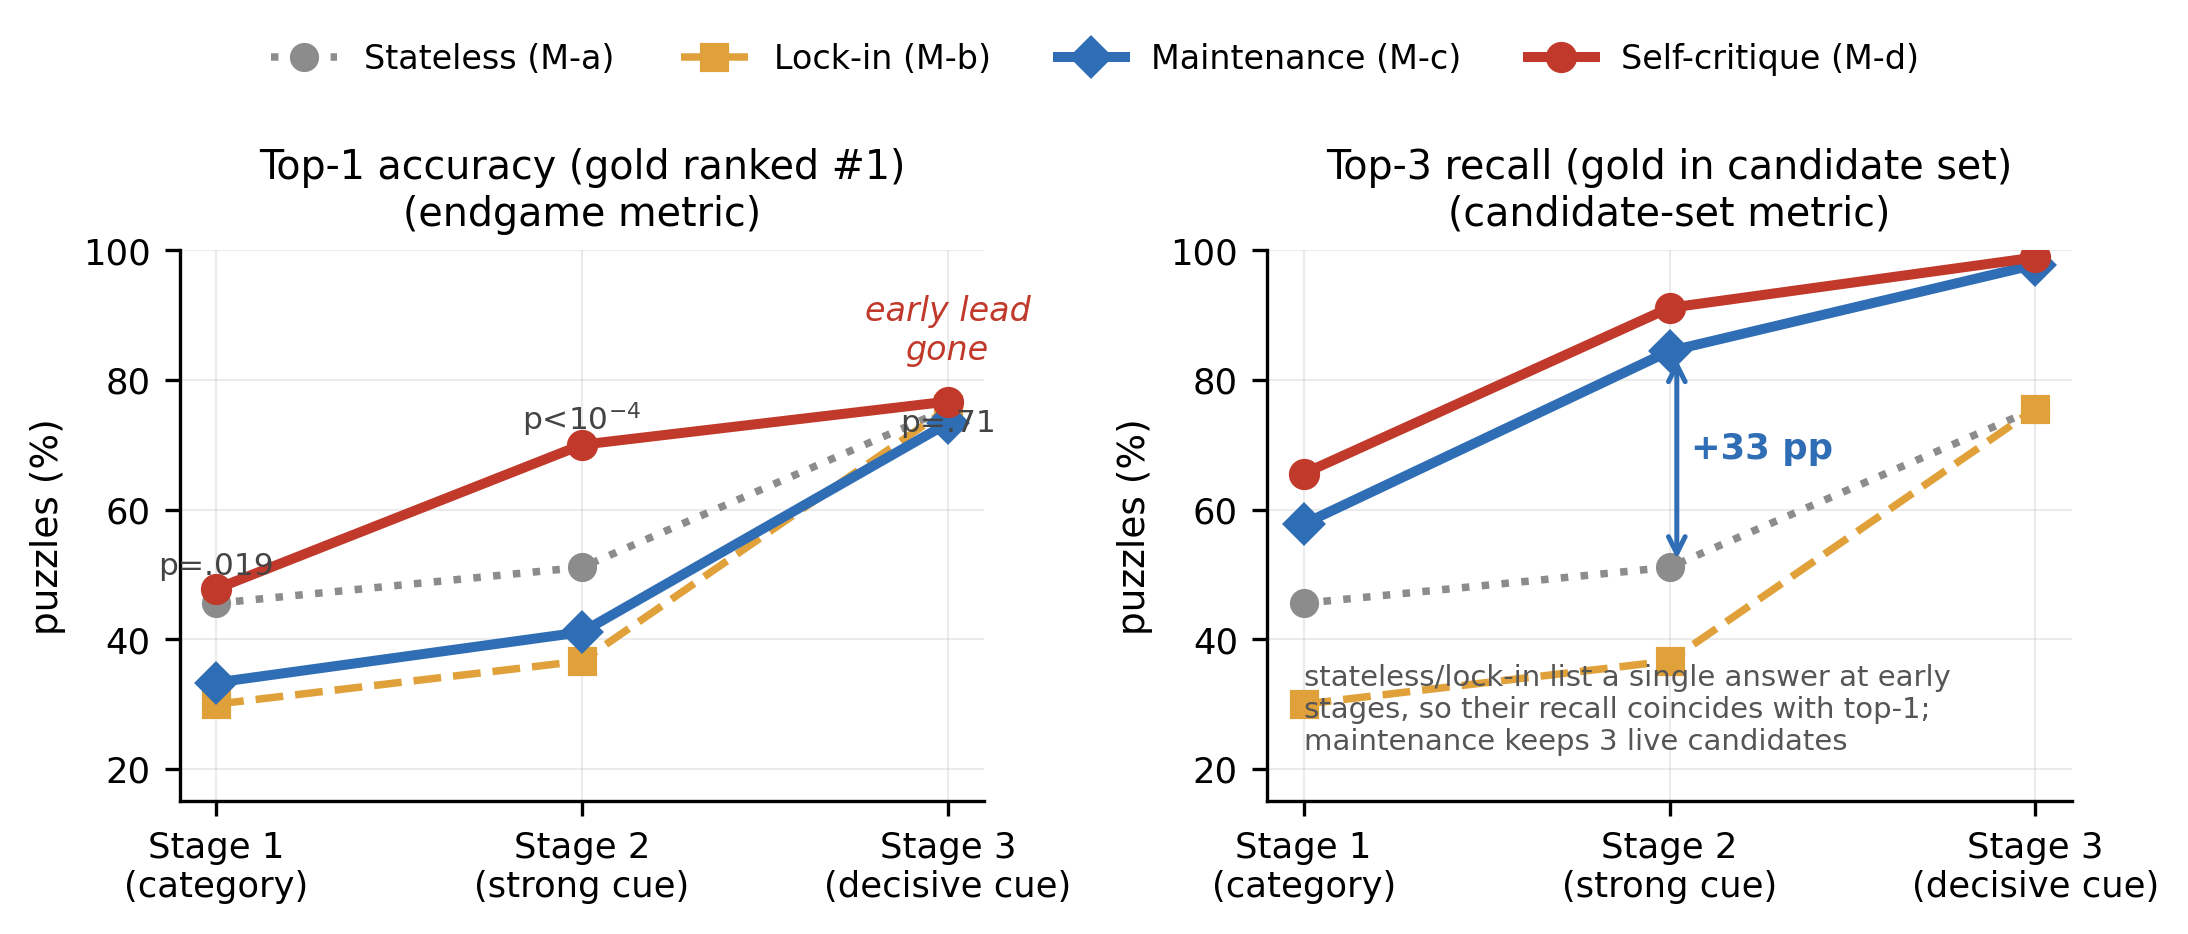
\includegraphics[width=\linewidth]{figs/fig_main.png}
\caption{The merged 90-puzzle race separates the two claims.
\textbf{(a)}~Endgame-metric trajectories (top-1 accuracy, gold ranked
first): self-critique (\Mcrit{}, red) leads significantly at stages 1--2
(paired sign tests vs.\ \Mmaint{}: $p = 0.019$, $p < 10^{-4}$) but the
lead vanishes at stage 3 ($p = 0.71$)---an early-convergence effect, not
a higher ceiling. \textbf{(b)}~Candidate-set recall (gold among the
three listed candidates): hypothesis maintenance (\Mmaint{}, blue) holds
a $+33$\,pp advantage over stateless (\Mstate{}) at stage 2, exactly
where evidence is thinnest. Statelessly prompted mechanisms list a
single answer at early stages, so their recall coincides with top-1;
maintenance keeps three live candidates, and its endgame recall ($98\%$)
is the highest of all mechanisms. All values: merged set, batch-1
puzzles at temperature 0, confirmation puzzles scored by median rank
over three temperature-0.7 resamples.}
\label{fig:race}
\end{figure}

\section{The hypothesis-maintenance effect}
\label{sec:maint}

The race's one robust positive deserves its own statement, because it is
the mirror image of feedback. \Mmaint{} is not a feedback mechanism: no
signal is routed backward, no output is critiqued. It is a
\emph{discipline}---maintain a ranked, confidence-annotated candidate set
and refuse premature convergence. Its measured benefits:
\begin{enumerate}
\item \textbf{Early recall}. Candidate-set recall at stages 1/2 is higher
  than every alternative: $+12/+33$\,pp over \Mstate{} on merged data,
  with the advantage concentrated exactly where evidence is thinnest.
  Under evidence scarcity, maintaining three live hypotheses is worth
  more than any amount of single-shot deliberation.
\item \textbf{Endgame parity without cost}. Unlike classic
  explore/exploit trade-offs, maintenance does not pay for its early
  breadth at the endgame: top-1 $73\%$ vs.\ \Mstate{}'s $76\%$ is within
  noise, and its \emph{top-3 recall} at the endgame ($98\%$) is the
  highest of all mechanisms---the candidate set it maintains stays honest
  even after convergence is licensed.
\item \textbf{A measurable failure mode that localizes it}. Maintenance's
  cost surface appears as \emph{placeholder duplication}: when evidence
  is overwhelming, \Mmaint{} fills its mandated three slots with the same
  gold answer at $99.9\%$ plus two sub-1\% decoys (16/30 batch-1 puzzles
  show $\ge 2$ duplicates). Instruction compliance (fill three slots)
  and semantic convergence (one answer) pull apart. Self-critique
  suppresses the duplication---the one concrete thing the critique round
  demonstrably does.
\end{enumerate}

\subsection{A $2\times2$ decomposition: format first, history second}
\label{sec:twobytwo}

\Mmaint{} differs from \Mstate{} in two ways at once: it keeps candidate
history in context, and it demands the three-candidate confidence format.
Which ingredient carries the early-recall benefit? We ran the missing
cells: \emph{format-only} (\Mstate{} prompt replaced by \Mmaint{}'s
first-turn prompt, standalone at each stage) and \emph{bare-history}
(\Mlock{}'s single-answer discipline with conversational updating), on
the 60 confirmation puzzles under the identical temperature and scoring
protocol (1080 additional queries).

\begin{table}[h]
\centering
\small
\begin{tabular}{lcccccc}
\toprule
 & \multicolumn{3}{c}{Recall (top-3)} & \multicolumn{3}{c}{Top-1} \\
\cmidrule(lr){2-4}\cmidrule(lr){5-7}
Arm & G1 & G2 & G3 & G1 & G2 & G3 \\
\midrule
\Mmaint{} (hist.+format) & 30 & 50 & 60 & 18 & 26 & 48 \\
format-only             & 30 & 32 & 47 & 22 & 23 & 43 \\
\Mlock{} (hist.+bare)    & 15 & 21 & 46 & 15 & 21 & 46 \\
bare (no hist., no fmt) & 23 & 22 & 44 & 23 & 22 & 44 \\
\bottomrule
\end{tabular}
\caption{The $2\times2$ on 60 confirmation puzzles (median rank over
3 resamples). Recall counts: gold among the three listed candidates.}
\label{tab:twobytwo}
\end{table}

The decomposition reverses the natural reading. The \emph{format main
effect is the larger one} ($+32$\,pp at stage 2; 41/1/18 win/tie/loss,
$p < 10^{-4}$): simply being asked to list three confidence-annotated
candidates nearly doubles early recall. The \emph{history main effect}
is $+14$\,pp ($p < 10^{-4}$), but it is entirely concentrated in the
format arm: $+30$\,pp with format, $-2$\,pp without (interaction $+32$\,pp,
$p = 10^{-4}$). At stage 1 the format-only arm already matches \Mmaint{}
exactly (30/60 each)---the format alone creates the candidate space;
history cannot be credited for stage-1 gains. What history buys is the
\emph{realization} of that space as evidence accumulates: with the
format demanding three live slots, the conversational record of prior
candidates lifts stage-2 recall from 32 to 50.

Placeholder duplication tells the same story from its failure side. It
is a cost of the \emph{format}, not of maintenance: format-only shows
$\ge 1$ duplicate on 18/60 puzzles (mean 0.57), history-less, and
\Mmaint{} roughly doubles it (36/60, mean 1.18); the bare arms
structurally never duplicate. The tension the duplication indexes
---comply-with-three vs.\ converge-on-one---belongs to the format;
history deepens rather than creates it.

We therefore restate the effect: \emph{the format builds the candidate
space; the history cashes it in}. Neither alone reproduces \Mmaint{}'s
early profile, and the abductively virtuous component---refusing
premature convergence under thin evidence---is present in the format
instruction itself, a much cheaper intervention than conversational
state. The endgame, as everywhere in this race, shows no meaningful
spread (top-1 $72$--$80\%$ across all four arms).

The alignment with the abduction literature
\citep{peirce1878abduction,josephson1996abductive,tenenbaum2011grow} is
direct, but the measurement is new: to our knowledge this is the first
preregistered, multi-batch quantification of the maintain-vs-commit
trade in an LLM. The $2\times2$ adds a twist the abduction frame does
not predict: the discipline lives mostly in the \emph{output format},
not the maintained state---asking for three ranked confidence-annotated
candidates buys $+18$\,pp of early recall by itself, and the
conversational record is the amplifier, not the engine
(\S\ref{sec:twobytwo}).

\section{Self-critique decomposed: early convergence, not a higher ceiling}
\label{sec:early}

Why did \Mcrit{} look like a winner in batch 1? Because its benefit is
real but mislocated in time. Pairing \Mcrit{} against \Mmaint{} on
endgame top-1 hides a strong stage-resolved effect:
\begin{itemize}
\item \textbf{Stage 1}: \Mcrit{} $43/90$ vs.\ \Mmaint{} $30/90$;
  paired 20 wins / 7 losses, sign test $p = 0.019$.
\item \textbf{Stage 2}: $63/90$ vs.\ $37/90$; 32 wins / 6 losses,
  $p < 10^{-4}$.
\item \textbf{Stage 3}: $69/90$ vs.\ $66/90$; 16 / 13, $p = 0.71$.
\end{itemize}
The critique round accelerates convergence: it pulls correct answers to
the top earlier in the evidence schedule. But the endgame ceiling is
identical---\Mmaint{} catches up once evidence suffices---so on an
endgame-scored task the apparent batch-1 advantage was timing misread as
accuracy. The difficulty gradient sharpens the point: on the 60
confirmation puzzles, \Mcrit{} vs.\ \Mmaint{} endgame deltas are $+17$\,pp
(hard), $-16$\,pp (medium), $-9$\,pp (easy). Where the candidate ordering
was already correct (medium/easy), critique perturbs it; where it was
wrong (hard), critique helps. Feedback's value tracks exactly the
states where the base mechanism is \emph{not} already converged---the
same lesson the collapse attractor taught on the CNN side, arrived at
from the opposite direction. One condition on these stage-resolved
numbers: they were measured under a 1{,}200-token output cap that
\Mcrit{} exhausted in 61\% of confirmation-batch calls, and when the cap
was raised to 2{,}400 for \Mcrit{} alone its top-1 was no higher at any
stage ($-1.7$, $-11.7$, $-13.3$\,pp; sign $p = 1.00$, $0.21$, $0.12$;
Limitations). The stage-2 lead is therefore a comparison made under the
binding budget, and the budget's effect on it is not resolved.

\section{The measurement artifact}
\label{sec:artifact}

A methodological note with general reach. Batch 1's first scorer counted
a gold answer's rank by the number of list markers preceding its
\emph{first textual occurrence}. Mechanisms \Mcrit{}/\Mmaint{} write an
analysis before their final list, and that analysis is itself often a
numbered list (``1.\ category clue; 2.\ second clue; 3.\ third clue'')
that names the gold answer in passing; the scorer counted those
enumeration markers and recorded a third-ranked list entry. The artifact
systematically favored \Mlock{} (which returns a bare answer with no
analysis) and manufactured part of the batch-1 anomaly (\Mlock{}
leading the endgame). A second artifact compounded it: a 400-token
output cap cut the long analyses mid-sentence before the candidate
list was reached. The repaired scorer anchors rank to \emph{structured
commitment positions}: lines that both carry a list marker and carry
(or are adjacent to) a confidence percentage, taking the
highest-confidence entry mentioning the gold answer. It also counts
\emph{duplicate} gold placements, which turned out to be a substantive
signal (\S\ref{sec:maint}, item 3). The lesson generalizes: when
comparing mechanisms with different output styles, score the position in
the output where the mechanism \emph{commits}, not where the string first
appears. All v1 batch data were discarded and re-run; both scorer
versions are archived.

\paragraph{Residual truncation, disclosed.}
Raising the cap to 1{,}200 tokens did not eliminate truncation; it made
it mechanism-specific. Replaying the archived scorer on the 360 batch-1
outputs gives zero rank mismatches, but a truncation census (output
longer than 800 characters and not ending on a sentence terminator)
finds 57.8\% of \Mcrit{} outputs cut mid-sentence, against 7.8\% for
\Mmaint{}, 4.4\% for \Mstate{}, and 0\% for \Mlock{}. The cut does not
reach the scored list---\Mcrit{} writes its revised candidates before
its closing commentary---and top-1 is unchanged between truncated and
complete \Mcrit{} outputs (65\% vs.\ 66\%). We therefore keep the
recorded ranks, but flag the asymmetry: \Mcrit{} alone was run under a
budget it routinely exhausted, so its early-convergence profile
(\S\ref{sec:early}) was measured under a constraint none of the other
mechanisms faced. A re-run of the confirmation batch with full texts
archived (same cap, same prompts) gives 61\% for \Mcrit{}, against 7\% for
\Mmaint{} and 2\% for \Mstate{}, now counted by the server's native
finish-reason flag rather than the heuristic; the pre-critique candidate
step was cut in only 7\% of \Mcrit{} calls, so the cut falls on the
critique pass itself. A further arm raised the cap to 2{,}400 tokens for
\Mcrit{} alone, which lowered the cut rate to 9\% (15\% at stage 3) and
moved its top-1 by $-1.7$, $-11.7$, and $-13.3$\,pp at stages 1/2/3.
None of these shifts passed the preregistered paired sign test
($p = 1.00$, $0.21$, $0.12$), so the truncation is not a demonstrated
behavioral confound; nor is it demonstrated to be harmless, since the
stage-2 and stage-3 shifts are larger than the gate's own 10\,pp margin
(\S\ref{sec:limitations}, \emph{Unequal output budget}).

\paragraph{Scorer tolerance, verified.}
The repaired scorer lets a candidate borrow a confidence percentage from
the next two lines, to accommodate the common ``\texttt{1.~answer} /
confidence'' layout. This could in principle let a numbered reasoning
step inherit the next candidate's percentage. On the batch-1 texts the
borrowing path touches 5 rows, all prose justifications attached to the
correct candidate, and changes no recorded rank; a stricter scorer that
demands the percentage on the candidate's own line would move 7 of 360
ranks, all in the lenient direction. The tolerance is load-bearing, not
a leak.

\section{Discussion}
\label{sec:discussion}

\paragraph{One lesson, two regimes.}
Program A shows feedback failing because the trained state has already
absorbed the stress distribution's preferred solution; Program B shows
feedback failing \emph{at the endgame} even in a training-free regime
where the model is free to listen. The failure modes are different---%
inverted belief responses vs.\ pure null effect---but the design moral is
the same: feedback's presumed value (correction) presupposes a state
worth correcting. In A that state never exists (it is collapsed); in B it
exists but \Mmaint{} has already extracted the available value by stage 3.

\paragraph{Where guided feedback might still work.}
Our gates do not outlaw feedback everywhere; they locate it. Critique
genuinely helps on hard puzzles ($+17$\,pp), where the pre-critique
candidate set is wrong, and genuinely accelerates convergence at
intermediate stages. A regime where evidence never saturates---%
open-ended investigation rather than a three-stage reveal---would score
the intermediate stages as the endgame and might legitimately favor
critique. Our claim is narrower: on tasks with an evidence-terminus,
feedback's speed benefit is invisible to endgame scoring, and its
accuracy effect inverts on already-correct instances.

\paragraph{The attractor as scope condition.}
The collapse attractor result is also a scope condition for the broader
stress-rack methodology: robustness evaluations that train on the stress
distribution measure the attractor's behavior, not the architecture's
feedback capacity. The scope condition has teeth because both post-hoc
repair routes are now empirically closed: an anti-collapse objective and
two data-route repairs (interleaving, curriculum) all fail to restore the
error signal once training has selected the collapsed solution
(\S\ref{sec:threeway}--\ref{sec:distrepair}). Any feedback claim tested
under occlusion-style training must therefore be gated \emph{before} the
claim, not repaired after it: $\rhoerr > 0$ is a cheap precondition (one
forward pass plus a short probe fit). We suggest it as a standard gate for
feedback papers in degraded-input regimes.

\paragraph{Preregistration carried real weight.}
Three of this paper's readings are gates or checks that \emph{blocked}
seductive alternatives: an inverted belief response that would have read
as a mechanism discovery with a sign error, a $+23$\,pp trend that
would have survived any fixed narrative, and a mid-training probe whose
single-seed reading suggested a clean-vs-curriculum divergence that two
further control seeds dissolved. The confirmation-batch design
(freeze the effect size, the test, and the CI condition before enlarging
the sample) cost one day of compute and converted a would-be false
positive into a clean negative with a power calculation explaining why.
Preregistration fixed the claim; only replication fixed the probe.

\section{Limitations}
\label{sec:limitations}

\textbf{One LLM, one size.} All Program-B results are one 27B instruction
model. The batch-1-to-confirmation sign reversal is within-model
evidence about sample size, not about model generality; the
hypothesis-maintenance effect and the early-convergence decomposition
should be replicated across at least one other family
(e.g.\ \citealp{gemma2024}) and one smaller size before any
universality claim. \textbf{Task breadth.} Graded-evidence-reveal puzzles
are short-horizon abduction with verifiable unique answers; they do not
exercise long-chain reasoning or external-tool feedback, where
self-correction's strongest published gains live. Our negative result
bounds the \emph{endgame} claim in a clean setting; it does not
adjudicate tool-augmented critique, where the feedback signal is external
ground truth rather than self-generated. \textbf{CNN side is one stress
family.} The attractor analysis covers occlusion grids; other stressors
(noise, blur, distribution shift) may not select collapse, and feedback might
show gains there. Our claim is that occlusion-trained racks---the exact
setting motivating most robustness feedback papers---carry the confound,
not that all stress racks do. \textbf{Repairs are two, not all.} The
distribution route was tested with exactly two interventions---1:1
interleaving and a fixed 30/30 clean-to-occluded schedule---and the
objective route with one consistency term. Our claim is that the obvious
post-hoc repairs fail, not that no data schedule could prevent the
attractor; earlier, gentler, or continuously annealed exposure to clean
data is untested. \textbf{Formation time is bracketed, not located.} The
signature is inverted by epoch 60; a mid-training probe (25-epoch probe
fit at epoch 30) returned seed-inconsistent values even in the
clean-training control (range $-1.00$ to $+0.96$ across three seeds) and
is not reliable enough to date the transition. \textbf{Scorer subjectivity.} The
confidence-anchored scorer depends on models emitting confidence-bearing
structured lists; models that refuse the format would need a different
commitment-position definition, and we cannot exclude scorer-model format
interactions at other scales. \textbf{Three resamples per cell.} Scoring the
confirmation batch by median rank over three temperature-0.7 resamples is
cheap but coarse: the median of three binary indicators moves by whole
puzzle counts. A re-run of the batch under identical prompts, temperature,
and cap (ADR-0034) left \Mcrit{}'s column of Table~\ref{tab:merged} within
one puzzle of the reported counts ($44/63/70$) but moved \Mmaint{}'s to
$33/46/60$ (reported $30/37/66$), so the merged endgame difference becomes
$+10$ puzzles and the stage-1 paired test $p = 0.07$ (reported $+3$ and
$p = 0.019$); stage 2 stays significant and the endgame stays null under
both draws. Table~\ref{tab:merged} reports the preregistered draw; the
stage-1 lead should be read as suggestive, not established, and the
per-puzzle instability sits in the control arm, which was not the subject
of the re-run. \textbf{Unequal output budget.} The
1{,}200-token cap truncated 58\% of \Mcrit{} outputs and under 8\% of
every other mechanism's in the batch-1 archive; the re-run of the
confirmation batch puts the figure for \Mcrit{} at 61\%, counted by the
server's native finish-reason flag. Ranks were unaffected, but
\Mcrit{}'s behavior was observed under a binding budget that the
others did not hit. We therefore re-ran \Mcrit{} with the cap raised to
2{,}400 tokens on the same 60 confirmation puzzles. This cuts the
truncation rate to 9\% without eliminating it (15\% at stage 3), so the
arm is budget-relaxed rather than budget-free. The preregistered gate
(a top-1 difference of at least 10\,pp at any stage \emph{and} a paired
sign test at $p < 0.05$) did not fire: top-1 moved by $-1.7$, $-11.7$,
and $-13.3$\,pp at stages 1/2/3, with $p = 1.00$, $0.21$, and $0.12$.
We read this as \emph{not detected}, not as \emph{no effect}. The
stage-2 and stage-3 differences are as large as the cap was expected to
produce and point the same way, the paired bootstrap intervals
($[-26.7, +3.3]$ and $[-26.7, +1.7]$\,pp) do not exclude a 10\,pp
effect, and the sign test sees only about 20 discordant puzzles per
stage. The relaxed arm also produced longer critiques that restated the
gold answer in more list entries (mean duplicate-gold count 0.73 vs.\
1.38 at stage 2, 0.96 vs.\ 1.89 at stage 3). On top-1 the relaxed arm
scored \Mcrit{} no higher at any stage, so if the cap biases \Mcrit{},
the bias runs in \Mcrit{}'s favor; only \Mcrit{} was re-run at the larger
budget, so the stage-2 lead in \S\ref{sec:early} remains a comparison
made under the binding budget.

\section{Conclusion}
\label{sec:conclusion}

Across a CNN stress rack and an LLM mechanism race, guided feedback
failed its preregistered endgame tests, and the two failures are
diagnosed rather than merely recorded: one competes with a trained
collapse attractor, the other dissolves into a timing effect with a
difficulty gradient. The replicable benefit belongs to hypothesis
maintenance---an instruction-level discipline that keeps candidate sets
honest under evidence scarcity, buys early recall at no endgame cost,
and needs no backward signal at all. For builders of robust perception
pipelines and self-improving reasoners alike, the cheap first question
is not ``how should feedback be wired'' but ``does the current state
still carry a correctable error signal''---and if it does, whether the
real scarcity is correction or simply the discipline of not
converging first.

\section*{Reproducibility statement}
All batches were preregistered with frozen criteria: the LLM race batches
under ADR-0029 through ADR-0032 (including the confirmation batch's
effect-size threshold, test, and CI condition, fixed before the 60 new
puzzles were generated and run, and the $2\times2$ decomposition's
main-effect gates), the truncation re-run and its relaxed-budget arm
under ADR-0034 (the top-1 difference and sign-test threshold fixed
before launch), and the distribution-intervention batch under
ADR-0033 (three arms, three seeds, reversal gates fixed before launch).
Puzzle generators, race scripts, scorer versions (including the
discarded first scorer), and analysis
notebooks are archived; batch-1 outputs with full texts (360 records),
per-query records for the confirmation batch (2160 queries: ranks,
duplicate counts, difficulty), and the $2\times2$ probe are
released as machine-readable JSON, as are the per-run probe
outputs for every training condition in Table~\ref{tab:attractor}.
The confirmation batch itself retained no full texts; a re-run of it
under ADR-0034 (same puzzles, prompts, and cap) archived them, and that
re-run is released in \texttt{results/p35\_fulltext} alongside the
per-query records, together with the 2{,}400-token \Mcrit{} arm and the
read-out scripts.
Bootstrap uses 20{,}000 resamples with a fixed seed.

\section*{Ethics statement}
This study uses publicly available model weights served locally and
synthetic text puzzles with no personal data; no human subjects were
involved. Negative results are reported to reduce community waste on
unpromising directions; we report power calculations alongside null
results to prevent over-reading them.

\section*{Use of AI tools}
Large language models were used as writing and coding assistants
(race-script implementation, scorer prototyping, and manuscript editing).
All scientific decisions---task design, frozen criteria, adjudications,
and every reported number---were determined by the authors and verified
against archived machine-readable records.

\bibliography{references}
\bibliographystyle{tmlr}

\appendix

\section{Batch-level detail and per-stage tables}
\label{app:tables}

\paragraph{Batch 1 (30 puzzles, temperature 0).}
Endgame top-1: \Mstate{} $23/30$, \Mlock{} $22/30$, \Mmaint{} $18/30$,
\Mcrit{} $25/30$. Early-stage recall (\Mmaint{} vs.\ \Mstate{}):
$73\%/87\%$ vs.\ $53\%/63\%$. Placeholder duplication (\Mmaint{}):
mean 1.70 duplicates at stage 3; 16/30 puzzles with $\ge 2$; negative
association with top-1 ($56\%$ vs.\ $64\%$ for high/low duplication).

\paragraph{Confirmation batch (60 new puzzles, temperature $0.7 \times 3$).}
2160 queries; median-rank scoring. Difficulty-stratified endgame deltas
(\Mcrit{} $-$ \Mmaint{}): hard $+2$ of 12 ($+17\%$), medium $-4$ of 25
($-16\%$), easy $-2$ of 23 ($-9\%$). Merged-set stage-resolved paired
sign tests (\Mcrit{} vs.\ \Mmaint{} top-1): stage 1 $p = 0.019$, stage 2
$p < 10^{-4}$, stage 3 $p = 0.71$.

\section{Scorer specification}
\label{app:scorer}

A candidate entry is a line carrying a list marker (numbered, bulleted,
or parenthesized) whose line or one of the two following lines contains a
confidence percentage. Rank of gold = position (within the candidate
sequence) of the \emph{highest-confidence} entry mentioning gold;
duplicates = count of additional entries mentioning gold. Absent gold
scores rank 0; API errors score $-1$ and are excluded from accuracy
denominators. The discarded v1 scorer (first-mention anchoring) and the
repair history are archived with the batch data.

\end{document}
